\chapter{САМОСТОЯТЕЛЬНАЯ СБОРКА РОБОТА}
\section{Обзор робота}
Данный робот -- отличная отправная точка для создания первого рабочего робота из
набора PRIME. Данный робот -- это базовый трехколесный робот, который быстро и легко
собирается и дает хорошее представление о внутренней работе основных конструктивных элементов и
элементов движения.

\section{Описание робота}
Робот использует один сервопривод непрерывного вращения в качестве приводного двигателя и один
стандартный сервопривод для рулевого управления в конструкции tri-bot. В качестве дополнительного варианта
к модели может быть добавлен захват TETRIX PRIME вместе с другим стандартным серводвигателем для захвата предметов.
\newpage
\section{Сборка робота}
\begin{figure}[h]
    \begin{subfigure}[b]{0.45\textwidth}
        \centering
        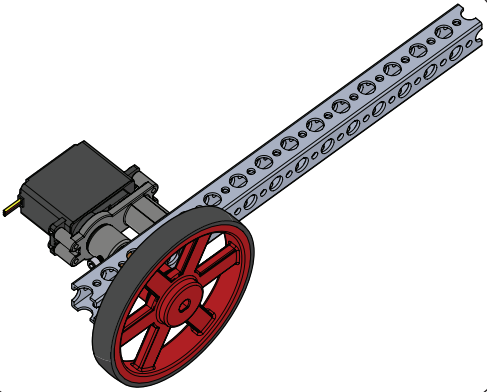
\includegraphics[width=0.7\textwidth]{fig/assembly/4.1.png}
        \caption*{Шаг 1}
    \end{subfigure}
    \begin{subfigure}[b]{0.45\textwidth}
        \centering
        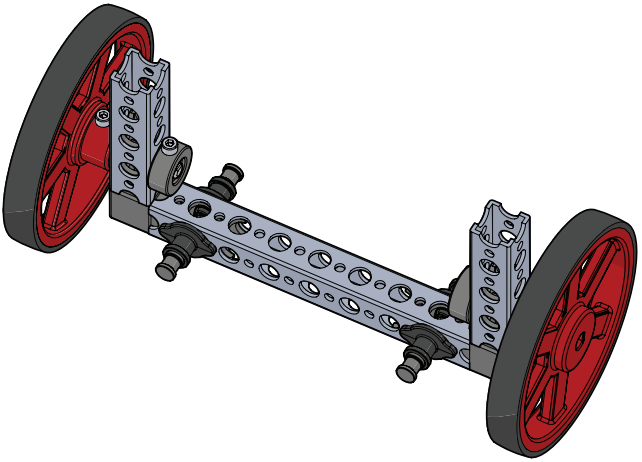
\includegraphics[width=0.7\textwidth]{fig/assembly/4.2.png}
        \caption*{Шаг 2}
    \end{subfigure}
    \begin{subfigure}[b]{0.45\textwidth}
        \centering
        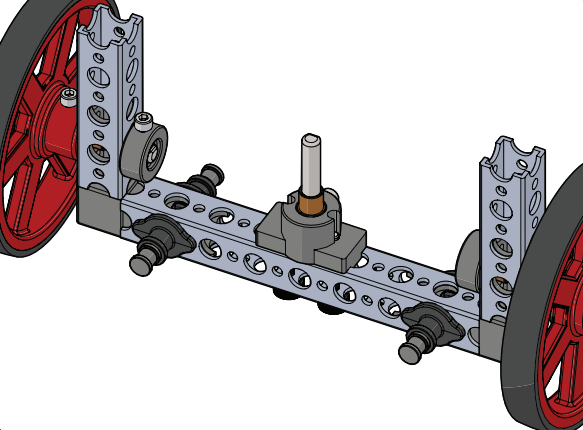
\includegraphics[width=0.7\textwidth]{fig/assembly/4.3.png}
        \caption*{Шаг 3}
    \end{subfigure}
    \begin{subfigure}[b]{0.45\textwidth}
        \centering
        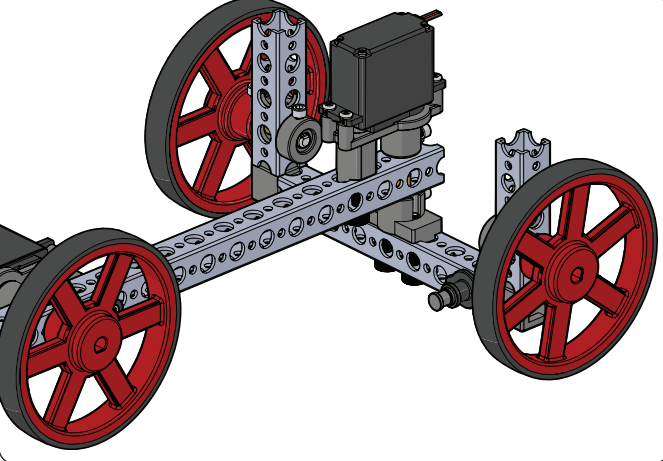
\includegraphics[width=0.7\textwidth]{fig/assembly/4.4.png}
        \caption*{Шаг 4}
    \end{subfigure}
    \begin{subfigure}[b]{0.45\textwidth}
        \centering
        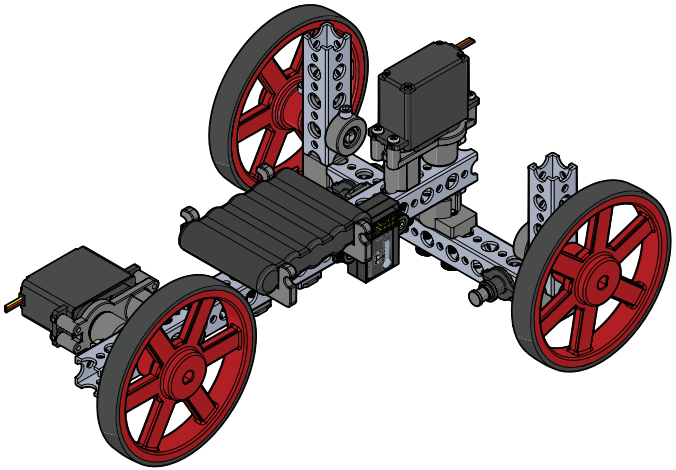
\includegraphics[width=0.7\textwidth]{fig/assembly/4.5.png}
        \caption*{Шаг 5}
    \end{subfigure}
    \begin{subfigure}[b]{0.45\textwidth}
        \flushright
        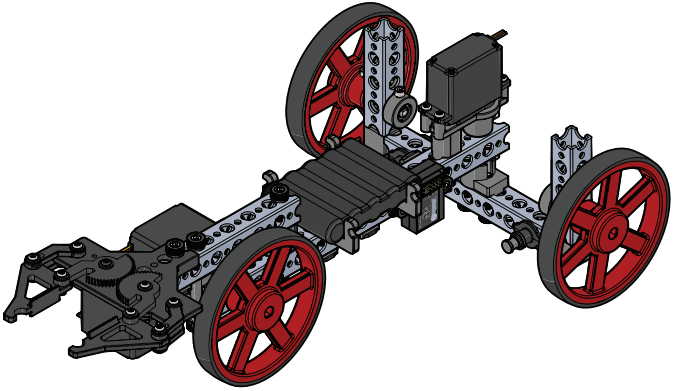
\includegraphics[width=0.7\textwidth]{fig/assembly/4.6.png}
        \caption*{Шаг 6}
    \end{subfigure}
\end{figure}

%\newpage
\section{Подключение робота}
Подключение робота представлено на рисунке \ref{4connect}.
\begin{figure}[hb]
    \centering
    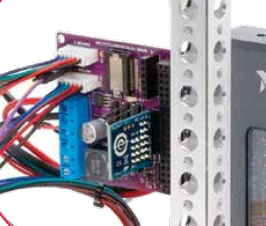
\includegraphics[width=0.3\textwidth]{fig/assembly/4.7.png}
    \caption{Подключение двигателей и периферии}
    \label{4connect}
\end{figure}

\newpage
\section{Испытание робота}
Управление роботом осуществлялось дистанционно.
Управляющая программа робота представлена на рисунке \ref{4prog}.
\begin{figure}[h]
    \centering
    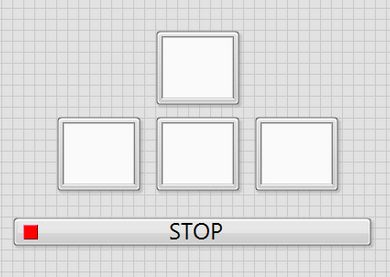
\includegraphics[width=0.7\textwidth]{fig/assembly/4.8.jpg}
    \caption{Реализация удаленного управления роботом}
    \label{4prog}
\end{figure}

\section{Устранение неисправностей}
\begin{itemize}
    \item Убедитесь, что стол, за которым вы работаете, ровный и неподвижный
    \item Убедитесь, что и myRIO, и аккумулятор надежно закреплены в системе, так как их вес способствует устойчивости
    \item Если у вас возникли проблемы с отправкой сообщений с вашего хост-компьютера в my ROOM, убедитесь, что IP-адрес на передней панели хост-устройства совпадает с IP-адресом myRIO wireless
    \item Дважды проверьте, правильно ли подключены двигатели и энкодер -- если их поменять местами, робот не будет балансировать
\end{itemize}
